\chapter{First Task}
This first set of images presents neither overlapping between objects nor distractors or noise, the only possible variation is in the backlighting's source power. 

In such a setting it's crucial to employ a robust algorithm to automatically
select a correct threshold for binarization.

Even though images have a bimodal histogram, foreground and background pixels have significantly different variances, and the application of Otsu's method for segmentation results in the wrong classification of rods' shadows, which in turn leads to the computation of inaccurate metrics.

I tried to employ a variation of the so-called "valley-emphasis method", proposed by Hui-Fuang et al.\cite{otsu_improved}, with poor results. 

Therefore I employed a more sophisticated, time-consuming method, which achieves the desired outcome. 

After approximating the probability density function of the pixels' intensity through gaussian kernel density estimation, the second zero-crossing of the first derivative of the pdf is found (the first zero-crossing corresponds to the first mode), which is the binarization's threshold.

For simplicity, I make use of a function provided by the library Scipy for relative minima computation after performing kernel density estimation.

The only parameter which has to be tuned is the bandwidth, which acts as a smoothing parameter controlling the bias-variance tradeoff (the higher the bandwidth, the smaller the variance), and which has been set to 6 for all the images in the dataset.
An example of binarization both with this method and with Otsu's method, can be seen in \ref{fig:thresholds}.

\vspace{7 mm}
\begin{figure}[h]
    \centering
    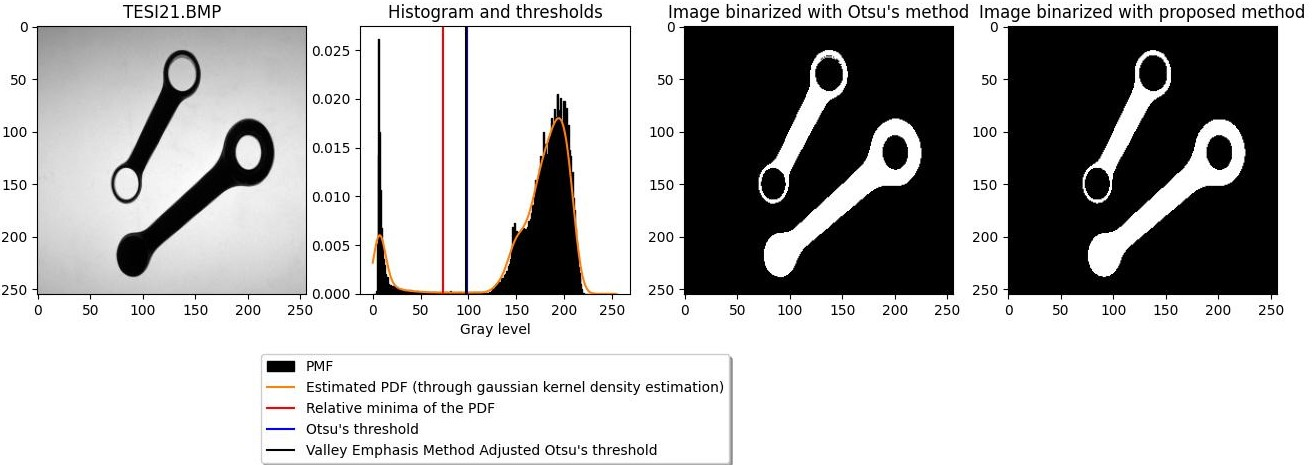
\includegraphics[scale=0.4]{tesi21_comparison.jpg}
    \caption{A comparison of the different thresholding methods.}
    \label{fig:thresholds}
\end{figure}

After binarization, the following operations are performed:
\begin{enumerate}
	\item Identification of connected components,
	\item Computation of minimum enclosing rectangles,
	\item Computation of descriptive statistics for the blobs, and the required metrics,
	\item Visualization of analysis results.
\end{enumerate}